\documentclass[8pt]{beamer}
\usefonttheme[onlymath]{serif}


\setbeamertemplate{frametitle}{%
  \vskip1ex
  \usebeamerfont{frametitle}%
  \insertsubsectionhead\par        %  ← 원하는 대로 변경 가능
  \vskip1ex
  \hrule                             % 밑줄(선택)
}

% 테마 선택 (선택 사항)
% \usetheme{Madrid} % 기본 테마, 다른 테마 사용 가능
% \font{serif}
\usepackage{amsfonts}
\usepackage{amssymb}
\usepackage[T1]{fontenc} % To use combination of textbf, textit
\usepackage[dvipsnames]{xcolor}   % can use more variant colors

% \setcounter{MaxMatrixCols}{20}

% (필요한 패키지들)
% \usepackage{amsthm}
\setbeamertemplate{theorems}[numbered]  % 정리, 정의 등에 번호를 달아줌

% \theoremstyle{plain} % insert bellow all blocks you want in italic
% \newtheorem{theorem}{Theorem}[section] % to number according to section
% 
% \theoremstyle{definition} % insert bellow all blocks you want in normal text
% \newtheorem{definition}{Definition}[section] % to number according to section
% \newtheorem*{idea}{Proof idea} % no numbered block

\newtheorem{proposition}[theorem]{Proposition}

\usepackage{tcolorbox}

% 필요할 경우 패키지 추가
\usepackage{graphicx} % 이미지 삽입을 위한 패키지
\usepackage{amsmath}   % 수식 사용
\usepackage{hyperref}  % 하이퍼링크 추가
\usepackage{cleveref}
\usepackage{multicol}  % 여러 열 나누기
\usepackage{ulem} % 취소선 및줄 나누기



\newcommand{\mrm}[1]{\mathrm{#1}}
\newcommand{\mbb}[1]{\mathbb{#1}}
\newcommand{\mb}[1]{\mathbf{#1}}
\newcommand{\mc}[1]{\mathcal{#1}}
\newcommand{\tb}[1]{\textbf{#1}}
\newcommand{\ti}[1]{\textit{#1}}
\newcommand{\Pois}[1]{\operatorname{Pois}(#1)}

\newcommand{\myber}[1]{\operatorname{Bern}\!\left(#1\right)}
\newcommand{\Bin}[2]{\operatorname{Bin}\!\left(#1,#2\right)}
\newcommand{\mytoinf}[1]{#1 \rightarrow \infty}
\newcommand{\myexp}[1]{\exp{\left(#1\right)}}
\newcommand{\myunif}[2]{\operatorname{Unif}\!\left(#1, #2\right)}
\newcommand{\mygeom}[1]{\operatorname{Geom}\!\left(#1\right)}
\newcommand{\Expo}[1]{\operatorname{Expo}\!\left(#1\right)}
\newcommand{\abs}[1]{\left\lvert #1 \right\rvert}
\newcommand{\expec}[1]{\operatorname{E}\left[ #1 \right]}
\newcommand{\Var}[1]{\operatorname{Var}\left[#1\right]}
\newcommand{\myskew}[1]{\operatorname{Skew}\!\left[#1\right]}
\newcommand{\mykurt}[1]{\operatorname{Kurt}\!\left[#1\right]}
\newcommand{\mywei}[2]{\operatorname{Wei}\!\left(#1, #2\right)}
\newcommand{\Span}[1]{\operatorname{Span}\!\left(#1\right)}
\newcommand{\Cov}[2]{\operatorname{Cov}\!\left(#1, #2\right)}
\newcommand{\intinfty}{\int_{-\infty}^\infty}
\newcommand{\Corr}[2]{\operatorname{Corr}\!\left(#1, #2\right)}
\newcommand{\Mult}[3]{\operatorname{Mult}_{#1}\!\left(#2, #3\right)}


% 발표 제목, 저자, 날짜 설정
\title{Probability: Joint Distributions}
\author{Gwanwoo Choi}
% \date{}

\begin{document}
% 표지 슬라이드
\begin{frame}
    \titlepage
\end{frame}

% % 목차 슬라이드
% \begin{frame}
%     \frametitle{Table of Contents}
%     \tableofcontents
% \end{frame}

\subsection{Joint, marginal and conditional}

\begin{frame}{.}
    \begin{definition}[Joint PDF]
        The \ti{joint} CDF of r.v.s $X$ and $Y$ is the function $F_{X,Y}$ given by
        \[
            F_{X,Y} (x,y) = P(X\leq x, Y \leq y)
        \]
        The joint CDF of $n$ r.v.s is defined analogously
    \end{definition}

    \begin{definition}[Joint PMF]
        The \ti{joint} PMF of discrete r.v.s $X$ and $Y$ is the function 
        \[p_{X,Y}(x,y) = P(X=x,Y=y)\]
        The joint PMF of $n$ r.v.s is defined analogously
    \end{definition}

    \begin{itemize}
        \item for all $x$ and $y$,  $0 \leq P(X=x,Y=y) \leq 1$
        \item $\sum_x \sum_y P(X=x,Y=y) = 1$
    \end{itemize}
\end{frame}

\begin{frame}{.}
    \begin{definition}[Marginal PMF]
        For discrete r.v.s $X$ and $Y$, the \ti{marginal} PMF of $X$ is 
        \[
            P(X=x) = \sum_y P(X=x,Y=y)
        \]
    \end{definition}
    Another way to obtain marginal PMF is using the joint CDF
    \[
        F_X(x) = P(X \leq x) = \lim_{y \rightarrow \infty} P(X\leq x, Y\leq y) = \lim_{y \rightarrow \infty} F_{X,Y} (x,y)
    \]

    \begin{definition}[Conditional PMF]
        For discrete r.v.s $X$ and $Y$, the \ti{conditional} PMF of $Y$ given $X = x$ is 
        \[
        P(Y=y |X=x) = \frac{P(X=x,Y=y)}{P(X=x)}
        \]
    \end{definition}

    Note that by Bayes' rule:
    \[
    P(Y=y|X=x) = \frac{P(X=x|Y=y) P(Y=y)}{P(X=x)}
    \]
\end{frame}

\begin{frame}{.}
    \begin{definition}[Independence of r.v.s]
        Random variables $X$ and $Y$ are \ti{independent} if for all $x$ and $y$,
        \[
            F_{X,Y} (x,y) = F_X(x) F_Y(y)
        \]
        If $X$ and $Y$ are discrete, this is equivalent to the conditions
        \[
        \begin{gathered}
            P(X=y,Y=y) = P(X=x)P(Y=y)\\
            P(X=x|Y=y) = P(X=x) \quad (P(Y=y) > 0)
        \end{gathered}
        \]
    \end{definition}
    \begin{example}[Chicken-egg]
        Suppose a chicken lays a random number of eggs, $N$, where $N\sim \Pois{\lambda}$. Each egg independently hatches with probability $p$ and fails to hatch with probability $q= 1 - p$. Let $X$ be the number of eggs that hatch and $Y$ the number that do not hatch, so $X+Y = N$. What is the joint PMF of $X$ and $Y$?
    \end{example}

    $X|N \sim \Bin{n}{p}$ and $Y|N \sim \Bin{n}{q}$. $P(X=i,Y=j) = \sum_{n=0}^\infty P(X=i,Y=j|N=n)P(N=n) = P(X=i,Y=j) = P(X=i,Y=j|N=i+j)P(N=i+j) = P(X=i|N=i+j)P(N=i+j)$.

    $P(X=i,Y=j) = P(X=i|N=i+j)P(N=i+j) = \binom{i+j}{i} p^i q^j e^{-\lambda} \lambda^{i+j} / (i+j)! = (e^{-\lambda p} (\lambda p)^i / i!)\cdot (e^{-\lambda q} (\lambda q)^{j} / j!) \implies X \sim \Pois{\lambda p}, Y \sim \Pois{\lambda q}$
\end{frame}

\begin{frame}{.}
    \begin{theorem}
        If $X\sim \Pois{\lambda p}, Y\sim \Pois{\lambda q}$, then $N=X+Y \sim \Pois{\lambda}$ and $X|N \sim \Bin{n}{p}$
    \end{theorem}
    \begin{theorem}
        If $N \sim \Pois{\lambda}$ and $X|N = n \sim \Bin{n}{p}$, then $X\sim \Pois{\lambda p }, Y = N-X \sim \Pois{\lambda q}$, and $X$ and $Y$ are independent
    \end{theorem}
    \begin{definition}[Joint PDF]
        If $X$ and $Y$ are continuous with joint CDF $F_{X,Y}$, their \ti{joint} PDF is the derivative of the joint CDF with respect to $x$ and $y$
        \[
            f_{X,Y}(x,y) = \frac{\partial^2}{\partial x \partial y} F_{X,Y}(x,y)
        \]
        $f_{X,Y} (x,y)$ should satisfy
        \begin{itemize}
            \item $f_{X,Y} (x,y) \geq 0$
            \item $\int_{-\infty}^\infty \int_{-\infty}^\infty f_{X,Y}(x,y) dx dy =1$
        \end{itemize}
    \end{definition}
    For a general region $A \subseteq \mbb{R}^2$, $P((X,Y)\in A) = \iint_{A} f_{X,Y} (x,y) dx dy$
\end{frame}

\begin{frame}{.}
    \begin{definition}[Marginal PDF]
        For continuous r.v.s $X$ and $Y$ with joint PDF $f_{X,Y}$, the \ti{marginal} PDF of $X$ is 
        \[
            f_X(x) = \int_{-\infty}^\infty f_{X,Y} (x,y) dx dy
        \]
    \end{definition}

    \begin{definition}[Conditional PDF]
        For continuous r.v.s $X$ and $Y$ with joint PDF $f_{X,Y}$, the \ti{conditional} PDF of $Y$ given $X=x$ is 
        \[
        \begin{cases}
            f_{Y|X}(y|x) = \frac{f_{X,Y}(x,y)}{f_X(x)}  = \frac{f_{X,Y}(x,y)}{\int_{-\infty}^\infty f_{X,Y}(x,y) dy} &\quad (f_X(x) > 0) \\ 
            f_{Y|X}(y|x) = 0 &\quad (f_X(x) = 0)
        \end{cases}
        \]
    \end{definition}
\end{frame}

\begin{frame}{.}
    \begin{theorem}[Continuous form of Bayes' rule and LOTP]
        For continuous r.v.s $X$ and $Y$, we have the following continuous form of Bayes' rule:
        \[
            f_{Y|X}(y|x) = \frac{f_{X|Y}(x|y)f_Y(y)}{f_X(x)} \quad (f_X(x)>0)
        \]
        And we have the following continuous form of the law of total probability
        \[
        f_X(x) = \int_{-\infty}^\infty f_{X|Y}(x|y) f_Y(y)dy
        \]
    \end{theorem}

    \begin{definition}[Independence of continuous r.v.s]
        Random variables $X$ and $Y$ are \ti{independent} if for all $x$ and $y$,
        \[
        F_{X,Y} (x,y) = F_X(x)F_Y(y)
        \]
        If $X$ and $Y$ are continuous with joint PDF $f_{X,Y}$, this is equivalent to
        \[
        \begin{gathered}
            f_{X,Y} = f_X(x)f_Y(y) \\
            f_{Y|X} = f_Y(y) \quad (f_X(x) > 0)
        \end{gathered}
        \]
    \end{definition}

    
\end{frame}

\begin{frame}{.}
    \begin{proposition}
        Suppose the joint PDF $f_{X,Y}$ of $X$ and $Y$ factors as 
        \[
        f_{X,Y}(x,y) = g(x) h(y)
        \]
        for all $x$ and $y$, where $g$ and $h$ are nonnegative functions.
        Then $X$ and $Y$ are independent.
    \end{proposition}
    \begin{proof}
        \[
    \begin{gathered}
        f_X(x) = g(x) \int_{-\infty}^\infty h(y) dy \\
        f_Y(y) = h(y) \int_{-\infty}^\infty g(x) dx \\
        f_X(x) f_Y(y) = g(x) h(y) \iint_{-\infty}^\infty g(x) h(y) dx dy = g(x) h(y) = f_{X,Y} (x,y)
    \end{gathered}
    \]
    \end{proof} 

    Note that $f_X(x) = \frac{g(x)}{\int_{-\infty}^\infty g(x)dx}$ and $f_Y(y) = \frac{h(y)}{\int_{-\infty}^\infty h(y) dy}$

\end{frame}

\begin{frame}{.}
    \begin{example}
    Let $(X,Y)$ be a completely random point in the unit disk $\{(x,y): x^2 + y^2 \leq 1\}$ with PDF 
    \[
    f_{X,Y}(x,y) =
    \begin{cases}
        \frac{1}{\pi}  & \text{if } x^2 + y^2 \leq 1\\
        0 & \text{otherwise}
    \end{cases}
    \]
    \begin{itemize}
        \item $X$ and $Y$ are not independent since $f_{X,Y}(\frac{\sqrt{3}}{2}, \frac{\sqrt{3}}{2}) = 0$ and $f_Y(\frac{\sqrt{3}}{2})f_Y(\frac{\sqrt{3}}{2})\neq 0$.
        \item $X$ and $Y$ are not independent, since larger value $\abs{X}$ restricts $Y$ to be a smaller range
        \item $f_X(x) = \int_{-\sqrt{1 - x^2}}^{\sqrt{1 - x^2}}\frac{1}{\pi} dy= \frac{2}{\pi} \sqrt{1 - x^2}, -1 \leq x \leq 1$. $f_{Y|X}(y|x) = \frac{f_{X,Y}(x,y)}{f_X(x)} = \frac{1/\pi}{2\sqrt{1 - x^2} /\pi} = \frac{1}{2\sqrt{1 - x^2}}, -\sqrt{1 - x^2} \leq y \leq \sqrt{1 - x^2}$ $\implies$ the fact that conditional PDF $f_{Y|X}(y|x)$ is not free of $x$ means $Y$ is not independent with $X$.
    \end{itemize}
    \end{example}
\end{frame}

\begin{frame}{.}
    \begin{example}[Comparing Exponentials of different rates]
        Let $T_1 \sim \Expo{\lambda_1}$ and $T_2 \sim \Expo{\lambda_2}$ be independent. 
        Find $P(T_1 < T_2)$. For example, $T_1$ could be the lifetime of a refrigerator and $T2$ could be the lifetime of a stove (if we are willing to assume Exponential distributions for these), and then $P(T_1<T_2)$ is the probability that the refrigerator fails before the stove. 
        We know that $\min{T_1, T_2} \sim \Expo{\lambda_1 + \lambda_2}$, which tells us about \ti{when} the first appliance failure will occur, but we may also want to know about \ti{which} appliance will fail first.
    \end{example}
    \[
        \begin{aligned}
            P(T_1< T_2) &= \int_{0}^\infty \int_0^{t_2} \lambda_1e^{-\lambda_1 t_1} \lambda_2 e^{-\lambda_2 t_2} dt_1 dt_2 
            = \int_0^\infty (1 - e^{-\lambda_1 t_2}) \lambda_2 e^{-\lambda_2 t_2} dt_2 \\
            &= 1 - \lambda_2\int_0^\infty e^{-(\lambda_1 + \lambda_2)t_2} dt_2 = 1- \frac{\lambda_2}{\lambda_1 + \lambda_2} = \frac{\lambda_1}{\lambda_1 + \lambda_2}
        \end{aligned}
    \]
\end{frame}

\begin{frame}{.}
    \begin{example}[Cauchy PDF]
        Let $X$ and $Y$ be i.i.d. $\mathcal{N}(0,1)$, and let $T = X/Y$. (We can define $T$ arbitrary in the case $Y=0$; the choice of how to define $T$ in that case has no effect on the distribution of $T$, since $P(Y=0)=0$.) The distribution of $T$ is a famous named distribution called the \tb{Cauchy} distribution. Find the PDF of $T$.
    \end{example}
    Note that $P\left(\frac{X}{Y} \leq t\right) = P(X \leq tY, Y>0) + P(X \geq tY, Y<0) = P(X\leq tY, Y>0) + P(X \leq -tY, Y<0) = P(X\leq t\abs{Y})$.
    \[
    \begin{aligned}
        F_T(t) &= P(T\leq t) = P\left(\frac{X}{Y} \leq t\right) = P(X \leq tY, Y>0) + P(X \geq tY, Y<0) \\
        &= \int_0^\infty \int_{-\infty}^{ty} \frac{1}{\sqrt{2\pi}} e^{-x^2/2}  dx \frac{1}{\sqrt{2\pi}}e^{-y^2/2}dy \\
        &+ \int_{-\infty}^0 \int_{ty}^{\infty} \frac{1}{\sqrt{2\pi}}e^{-x^2/2} dx \frac{1}{\sqrt{2\pi}} e^{-y^2/2} dy \\ 
        &= \int_{-\infty}^\infty \int_{-\infty}^{t\abs{y}} \frac{1}{\sqrt{2\pi}}e^{-x^2/2} dx \frac{1}{\sqrt{2\pi}} e^{-y^2/2} dy = \frac{2}{\sqrt{2\pi}}\int_0^\infty \Phi(ty)  e^{-y^2/2} dy
    \end{aligned}
    \]
\end{frame}

\begin{frame}{.}
    \[
    \begin{aligned}
        f_T(t) &= F_T^\prime(t) = \frac{2}{\sqrt{2\pi}} \int_0^\infty \frac{\partial}{\partial t} \Phi(ty) e^{-y^2/2} dy \\
        &=  \frac{2}{\sqrt{2\pi}} \int_0^\infty y \frac{1}{\sqrt{2\pi}}e^{-(ty)^2/2} e^{-y^2/2} dy = \frac{1}{\pi} \int_0^\infty y e^{-(t^2 +1)y^2/2} dy \\
        &= \frac{1}{\pi (1+t^2)} \left[ e^{-(t^2 +1)y^2/2} \right]^0_\infty = \frac{1}{\pi (1+t^2)}
    \end{aligned}
    \]
    And $F_T(t) = \int_{-\infty}^t \frac{1}{\pi(1+t^2)} = \frac{1}{\pi} \operatorname{arctan}(t) + \frac{1}{2}$.

    An interesting fact about cauchy distribution is that although the PDF is symmetric about $0$, its expected value does not exist, since the integral $\int_{-\infty}^\infty \frac{t}{\pi(1+t^2)}dt$ diverges. For large $t$, $\frac{t}{1+t^2} \approx \frac{1}{t}$, and $\int^\infty_1 \frac{1}{t} dt = \infty$

\end{frame}

\begin{frame}{.}

    Suppose $X$ is \ti{discrete} r.v and $Y$ is \ti{continuous} r.v. Then \ti{marginal} distribution is defined by
    \[
        \begin{gathered}
            P(X=x) = \int_{-\infty}^\infty f_{X,Y}(X=x,y) dy\\
            f_Y(y) = \sum_x f_{X,Y}(X=x,y)
        \end{gathered}
    \]
    Conditional r.v. $X|Y$ and $Y|X$ are defined by
    \[
        \begin{gathered}
            P(X=x|y) = \frac{f_{X,Y}(X=x,y)}{\sum_x f_{X,Y} (X=x, y)} = \frac{f_{X,Y} (X=x,y)}{f_Y(y)} \\
            f_{Y|X} (y|X=x) = \frac{f_{X,Y}(X=x,y)}{\int_{-\infty}^\infty f_{X,Y}(X=x,y) dy} = \frac{f_{X,Y}(X=x,y)}{P(X=x)}
        \end{gathered}
    \]
    Bayes' rules are defined by 
    \[
        \begin{gathered}
            P(X=x|y) = \frac{f_{Y|X}(X=x,y) P(X=x)}{f_Y(y)}\\
            f_{Y|X}(y|X=x) = \frac{P(X=x|y)f_Y(y)}{P(X=x)}
        \end{gathered}
    \]
\end{frame}

\begin{frame}{.}
    \begin{example}
      A lightbulb was manufactured by one of two companies. 
      Bulbs that are made by Company 0 last an $\Expo{\lambda_0}$ amount of time, and bulbs made by Company 1 last an $\Expo{\lambda_1}$ amount of time, with $\lambda_0 < \lambda_1$. 
      The bulb of interest here was made by Company 0 with probability $p_0$ and by Company 1 with probability $p_1 = 1 - p_0$, but from inspecting the bulb we don't know which company made it.

      Let $T$ be how long the bulb lasts, and $I$ be the indicator of it having been made by Company 1.
      \begin{enumerate}
        \item Find the CDF and PDF of $T$.
        \item Does $T$ have the memoryless property?
        \item Find the conditional distribution of $I$ given $T=t$. What happens to this as $t \rightarrow \infty$?
      \end{enumerate}
    \end{example}
    1. $F_{T}(t) = P(T\leq t) = P(T\leq t|I=0)P(I=0) + P(T\leq t|I=1)P(I=1) = p_0 (1 - e^{-\lambda_0 t} )   + p_1 ( 1- e^{\lambda_1 t} ) = 1 - p_0 e^{-\lambda_0 t} - p_1 e^{-\lambda_1 t}, \forall t>0$. 
    $f_T(t) = \lambda_0 p_0 e^{-\lambda_0 t} + \lambda_1 p_1 e^{-\lambda_1 t}, \forall t>0$.

    2. No. because the distribution of $T$ is not Exponential.

    3.$P(I=1|t) = \frac{f_{T|I}(t|I=1) P(I=1)}{f_T(t)} = \frac{\lambda_1 p_1 e^{-\lambda_1 t}}{\lambda_0 p_0 e^{-\lambda_0 t} + \lambda_1 p_1 e^{-\lambda_1 t}}$. $t\rightarrow \infty$, then $P(I=1|t) \rightarrow 0$, which implies that the longer the bulb lasts, the more confident we will be that it was made by company 0
\end{frame}

\subsection{2D Lotus}

\begin{frame}{.}
    \begin{theorem}[2D LOTUS]
        Let $g$ be a function that $g: \mbb{R}^2 \rightarrow \mbb{R}$. If $X$ and $Y$ are discrete, then 
        \[
            \expec{g(X,Y)} = \sum_x \sum_y g(x,y) P(X=x,Y=y)
        \]
        If $X$ and $Y$ are continuous with joint PDF $f_{X,Y}$, then
        \[
            \expec{g(X,Y)} = \int_{-\infty}^\infty \int_{-\infty}^\infty g(x,y) f_{X,Y} (x,y) dx dy
        \]
    \end{theorem}

    \begin{example}
        Let $X$ and $Y$ be i.i.d. $\myunif{0}{1}$ r.v.s. Find $\expec{\abs{X-Y}}$
    \end{example}
    \[
    \begin{aligned}
        \expec{\abs{X-Y}} &= \int_0^1 \int_0^1 \abs{x-y} dx dy = \int_0^1 \int_y^1 (x-y)dx dy + \int_0^1 \int_0^y (y-x) dx dy \\
        &= 2 \int_0^1 \int_y^1 (x-y) dx dy = \frac{1}{3}
    \end{aligned}
    \]

\end{frame}

\begin{frame}{.}
    \begin{example}
        For $X, Y \overset{\text{i.i.d}}{\sim} \mc{N}(0,1)$. Find $\expec{\abs{X-Y}}$.
    \end{example}
    \[
    \expec{\abs{X-Y}} = \int_{-\infty}^\infty \int_{-\infty}^\infty \abs{x-y} \frac{1}{2\pi} e^{-(x^2 +y^2)/2}dxdy
    \]
    Calculate this. or another simple solution is using $X-Y = \sqrt{2}Z \sim \mc{N}(0, 2) (\because X+Y \sim \mc{N}(\mu_1 + \mu_2, \sigma_1^2 + \sigma_2^2)) $.

    \[
        \expec{\abs{X-Y}} = \sqrt{2}\expec{\abs{Z}} = \frac{2}{\pi}
    \]

    \begin{proposition}[Linearity via 2D LOTUS]
        Let $X$ and $Y$ be continuous r.v.s (the analogous method also works in the discrete case). By 2D LOTUS,
        \[
        \begin{aligned}
            \expec{(X+Y)} &= \int_{-\infty}^\infty (x+y)f_{X,Y}(x,y)dx dy \\
            &=\int_{-\infty}^\infty \int_{-\infty}^\infty x f_{X,Y}(x,y) dxdy + \int_{-\infty}^\infty \int_{-\infty}^\infty y f_{X,Y} dxdy \\ 
            &= \int^{\infty}_{-\infty} x \int_{-\infty}^\infty f_{X,Y} (x,y) dy dx + \int_{-\infty}^\infty y \int^{\infty}_{-\infty} f_{X,Y} (x,y) dx dy \\
            &= \expec{X} + \expec{Y}
        \end{aligned}
        \]
    \end{proposition}
\end{frame}
\subsection{Covariance and correlation}

\begin{frame}{.}
    \begin{definition}[Covariance]
        The \tb{covariance} between r.v.s $X$ and $Y$ is 
        \[
            \Cov{X}{Y} = \expec{(X - \expec{X})(Y - \expec{Y})} = \expec{XY} - \expec{X}\expec{Y}
        \]
        \begin{itemize}
            \item If $X$ and $Y$ are independent, then their covariance is zero. 
            \item We say that r.v.s with zero covariance are \tb{uncorrelated} $(\expec{XY} = \expec{X}\expec{Y})$.
        \end{itemize}
    \end{definition}

    \begin{theorem}
        If $X$ and  $Y$ are independent, then they are uncorrelated. (Converse is false)
    \end{theorem}

    \begin{proof}
        \[
        \begin{aligned}
            \expec{XY} &= \int_{-\infty}^\infty \int_{-\infty}^\infty xy f_{X,Y}(x,y) dx dy = \int_{-\infty}^\infty xy f_X(x)f_Y(y) dx dy \\
            &= \intinfty y f_Y(y) \left(\intinfty x f_X(x) dx \right) dy = \intinfty xf_X(x) dx \intinfty y f_Y(y) dy\\
            &=\expec{X}\expec{Y}
        \end{aligned}
        \]

        Converse is false. Let $Y = X^2, X \sim \mc{N}(0,1)$. Then $\expec{XY} = \expec{X^3} = 0$ and $\expec{x}\expec{y}= 0$. But $X$ and $Y$ are dependent.
    \end{proof}
\end{frame}

\begin{frame}{.}
    \begin{columns}
        \begin{column}{0.4\textwidth}
            Covariance is a measure of \tb{linear association}, so r.v.s can be dependent in nonlinear ways and still have zero covariance like in example $Y = X^2, X \sim \mc{N}(0,1)$
            \begin{itemize}
                \item $X$ and $Y$ is dependent in nonlinear ways and still have zero covariance.
                \item Bottom right plot of figure shows draws from the joint distribution of $X$ and $Y$.
            \end{itemize}
        \end{column}
        \begin{column}{0.6\textwidth}
            \begin{figure}
                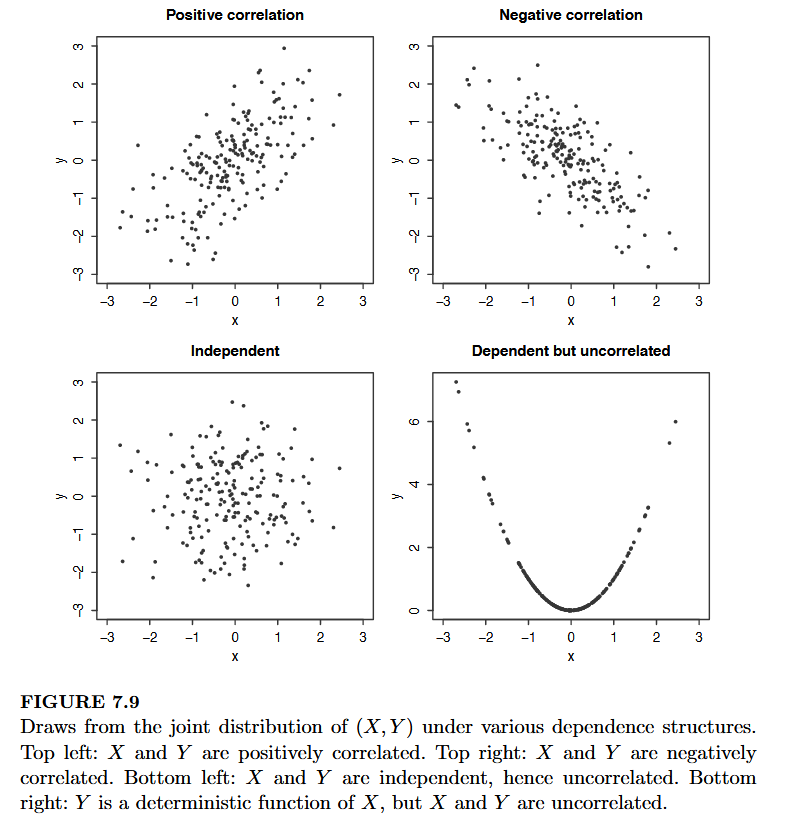
\includegraphics[width=1.0\textwidth]{CorrelateFigures.png}
            \end{figure}
        \end{column}
    \end{columns}
\end{frame}

\begin{frame}{.}
    Covariance has the following key properties

    \begin{enumerate}
        \item $\Cov{X}{X} = \Var{X}$
        \item $\Cov{X}{Y} = \Cov{Y}{X}$
        \item $\Cov{X}{c} = 0, \forall c \in \mbb{R}$
        \item $\Cov{aX}{Y} = a\Cov{X}{Y}, \forall a \in \mbb{R}$
        \item $\Cov{X+Y}{Z}=\Cov{X}{Z}+\Cov{Y}{Z}$
        \item $\Cov{X+Y}{Z+W} = \Cov{X}{Z}+\Cov{Y}{Z}+\Cov{X}{W}+\Cov{Y}{W}$
        \item $\Var{X+Y} = \Var{X}+\Var{Y}+2\Cov{X}{Y}$
        $= \Cov{X+Y}{X+Y} = \Cov{X}{X}+ \Cov{Y}{Y} + 2\Cov{X}{Y}$
    \end{enumerate}

    \begin{proposition}
        For independent r.v.s, the variance of the sum is the sum of the variances
        \[
            \Var{\sum_{j=1}^n X_j} = \sum_{j=1}^n \Var{X_j} 
        \]
    \end{proposition}
    \[
    \Cov{\sum_{j=1}^n X_j}{\sum_{i=1}^n X_j} = \sum_{j=1}^n \sum_{i=1}^n\Cov{X_j}{X_i} = \sum_{j=1}^n \Cov{X_j}{X_j}
    \]
\end{frame}

\begin{frame}{.}
    \begin{definition}[Correlation]
        The \tb{correlation} between r.v.s $X$ and $Y$ is
        \[
            \Corr{X}{Y} = \frac{\Cov{X}{Y}}{\sqrt{\Var{X} \Var{Y}}}
        \]
        This is only defined when $\Var{X} \neq 0$ and $\Var{Y} \neq 0$.
    \end{definition}
    For any constant $c$,
        \[
            \Corr{cX}{Y} = \frac{c\Cov{X}{Y}}{\sqrt{c^2 \Var{X}}{\Var{Y}}} = \Corr{X}{Y}
        \]
\end{frame}

\begin{frame}{.}
    \begin{theorem}[Correlation bounds]
        For any r.v.s $X$ and $Y$,
        \[
        -1 \leq \Corr{X}{Y} \leq 1
        \]
    \end{theorem}
    \begin{proof}
        Let $X$ and $Y$ be r.v.s s.t. $\Var{X} =1$ and $\Var{Y} =1$. Let $\rho = \Corr{X}{Y} = \Cov{X}{Y}$
        \[
        \begin{aligned}
            \Var{X+Y} \geq 0 \implies \Var{X} + \Var{Y} + 2\rho \geq 0 \implies -1\leq \rho\\
            \Var{X-Y} \geq 0 \implies \Var{X}+\Var{Y} - 2\rho \geq 0 \implies \rho \leq 1 \\
            \therefore -1 \leq \rho \leq 1
        \end{aligned}
        \]
    \end{proof}
\end{frame}

\begin{frame}{.}
    \begin{example}[Exponential max and min]
        Let $X$ and $Y$ be i.i.d. $\Expo{1}$ r.v.s. Find the correlation between $\max{(X,Y)}$ and $\min{(X,Y)}$.
    \end{example}

    Let $M = \max{(X,Y)}$ and $L = \min{(X,Y)}$. $L \sim \Expo{2}$ because $P(L \leq t) = P(X < t) + P(Y\leq t) = 1 - P(X>t, Y>t) = 1 - e^{-t} e^{-t} = 1- e^{-2t}, P(L = t) = 2e^{-2t}\implies L \sim \Expo{2}$.

    By memoryless property, $M-L \sim \Expo{1}$.

    \[
        \Cov{M}{L} = \Cov{M-L + L}{L} = \Cov{M-L}{L} + \Var{L} = \Var{L} =\frac{1}{4}
    \]
    \[
        \Var{M} = \Var{M-L+L} = \Var{M-L} + \Var{L} = 1+ \frac{1}{4} = \frac{5}{4}
    \]

    \[
        \Corr{M}{L} = \frac{\Var{L}}{\sqrt{\Var{M}}\Var{L}} = \frac{\sqrt{\Var{L}}}{\sqrt{\Var{M}}} = \frac{1}{\sqrt{5}}
    \]

\end{frame}

\subsection{Multinomial}

\begin{frame}{.}
    Each of $n$ objects is independently placed into one of $k$ categories. An object is placed into category $j$ with probability $p_j$. Let $X_1$ be the number of objects in category 1, $X_2$ the number of objects in category 2, etc., so that $X_1 + \cdots + X_k = n$. Then $\mb{X} = (X_1, \dots, X_k)$ is said to have the \tb{Multinomial distribution} with parameters $n$ and $\mb{p} = (p_1, \dots, p_k)$. We write this as $\mb{X} \sim \Mult{k}{n}{\mb{p}}$.

    We call $\mb{X}$ a \tb{random vector} because it is a vector of random variables.

    \begin{theorem}[Multinomial joint PMF]
        If $\mb{X} \sim \Mult{k}{n}{\mb{p}}$, then the joint PMF of $mb{X}$ is 
        \[
        P(X_1 = n_1, \dots, X_k=n_k) = \frac{n!}{n_1! n_2!,\dots, n_k!}\cdot p_1^{n_1} p_2^{n_2} \cdots p_k^{n_k}
        \]
        Where $n_1 + \cdots + n_k = n$.
    \end{theorem}

    \begin{theorem}[Multinomial marginals]
        The marginals of a Multinomial are Binomial. Specifically, if $\mb{X} \sim \Mult{k}{n}{\mb{p}}$, then $X_j \sim \Bin{n}{p_j}$.
    \end{theorem}
\end{frame}

\begin{frame}{.}
    \begin{theorem}[Multinomial lumping]
        \begin{itemize}
            \item If $\mb{X} \sim \Mult{k}{n}{\mb{p}}$, then for any distinct $i$ and $j$, $X_i + X_j \sim \Bin{n}{p_i + p_j}$.
            \item The random vector of counts obtained from merging categories $i$ and $j$ is still Multinomial. For example, merging categories $1$ and $2$ gives
            \[
                (X_1 +X_2, X_3, \dots, X_k) \sim \Mult{k-1}{n}{(p_1+ p_2, p_3, \dots, p_k)}
            \]
        \end{itemize}
    \end{theorem}

    Suppose $X_1 = n_1$ is observed. In that situation, what is the probability of $X_2 =n_2, \dots, X_k = n_k$?

    \[
        P(X_2 = n_2, \dots, X_k = n_k| X_1 = n_1) = \frac{P(X_1=n_1, \dots, X_k=n_k)}{P(X_1 = n_1)}
    \]

    What is the probability that one is in category $j$ given it is not in category $1$?
    \[
    P(\text{in category }j|\text{not in category }1) = \frac{P(\text{in category }j)}{P(\text{not in category }1)}
    \]
    \begin{theorem}[Multinomial conditioning]
        If $\mb{X} \sim \Mult{k}{n}{\mb{p}}$, then 
        \[
            (X_2, \dots, X_k)|X_1 =n_1 \sim \Mult{k}{n-n_1}{(p_2/z, \dots, p_k/z)}
        \]
        Where $z = p_2 + \cdots + p_k$
    \end{theorem}
\end{frame}

\begin{frame}{.}
    We already know that components within a Multinomial random vectors are dependent since $X_1 + \cdots + X_k = n$.
    \begin{theorem}[Covariance in a Multinomial]
        Let $(X_1, \dots, X_k) \sim \Mult{k}{n}{\mb{p}}$. For $i\neq j, \Cov{X_i}{X_j} = -n p_i p_j$ 
    \end{theorem}
    \begin{proof}
        $\forall i, j, i \neq j, X_i \sim \Bin{n}{p_i},X_j \sim \Bin{n}{p_j}, X_i +X_j \sim \Bin{n}{p_i + p_j}$. 
        \[
        \begin{aligned}
            &\Var{X_i + X_j} = \Var{X_i} + \Var{X_j} + 2\Cov{X_i}{X_j} \\
            \implies& n (p_i + p_j) (1 - p_i - p_j) = n p_i (1- p_i) + n p_j (1- p_j) + 2\Cov{X_i}{X_j} \\
            \implies&   -np_i p_j = \Cov{X_i}{X_j}
        \end{aligned}
        \]
    \end{proof}
\end{frame}

\begin{frame}{.}
    \begin{example}[Statwoman]
        The superhero Statwoman uses probability and statistics to fight crime. She has battled with countless foes, sometimes even fighting several at the same time. For simplicity though, assume that each of her battles is with exactly one of the following adversaries: the Confounder, the Extrapolator, and the Overfitter.

        Suppose that Statwoman will have $n$ battles next year (with $n$ a positive integer), and that each battle is with the Confounder with probability $p_1$, the Extrapolator with probability $p_2$, and the Overfitter with probability $p_3$, independently. Let $X_1, X_2, X_3$ be the numbers of battles Statwoman will have with the Confounder, the Extrapolator, and the Overfitter next year, respectively.

        \begin{itemize}
        \item Suppose for this part only that the parameters $p_1, p_2, p_3$ are \ti{unknown}, $n=360$, and it is observed that exactly $36$ of Statwoman's battles are with the Overfitter. A natural way to estimate $p_3$ is the value of $p_3$ that makes the observed data, $X_3 = 36$, as likely as possible. That is, the MLE is the value of $p_3$ that maximizes $P(X_3=36)$. Show that the MLE is the natural to estimate, 0.1.
        \end{itemize}

        $X_3 \sim \Bin{n}{p_3}, P(X_3 = x) = \binom{n}{x} p_3^x (1-p_3)^{n-x} = \frac{n!}{x! (n-x)!}p_3^x (1-p_3)^{n-x}$. 
        $\log{P(X_3=x)} = \log{n!} - \log{x!} - \log{(n-x)!} + x\log{p_3} + (n-x)\log{(1-p_3)}$

        $\frac{d \log{P(X_3=x)}}{dp_3} = \frac{x}{p_3} - \frac{n-x}{1-p_3}$. 
        Since $\frac{d^2 log{P(X_3=x)}}{dp_3^2} = -\frac{x}{p_3^2} - \frac{n-x}{(1-p_3)^2} < 0$,  $\hat{p_3}$ s.t. $\frac{x}{\hat{p_3}} - \frac{n-x}{1 - \hat{p_3}}= 0$ maximizes $P(X_3=x)$. By putting $x=36, n=360$, $\frac{36}{\hat{p_3}} - \frac{360 - 36}{1 - \hat{p_3}} = 0 \implies p_3 = 0.1$
    \end{example}
\end{frame}

\begin{frame}{.}
    \begingroup
        \setbeamercolor{itemize item}{fg=OliveGreen}
        \begin{itemize}
            \item Now suppose that, instead of the number of battles being a constant $n$, the number of battles is $N \sim \Pois{\lambda}$. Find the joint distribution of $X_1, X_2, X_3$.
        \end{itemize}
    \endgroup

    \[
    \begin{aligned}
        &P(X_1=n_1, X_2=n_2, X_3=n_3) \\
        &= \sum_{n=0}^\infty P(X_1=n_1, X_2=n_2, X_3=n_3 | N=n)p(N=n) \\
        &=P(X_1=n_1, X_2=n_2, X_3=n_3 | N=n_1+n_2+n_3)p(N=n_1+n_2+n_3) \\
        &=\frac{(n_1 + n_2 + n_3)!}{n_1! n_2! n_3!} p_1^{n_1} p_2^{n_2} p_3^{n_3} \frac{\lambda^{(n_1 + n_2 + n_3)}}{(n_1 + n_2 + n_3)!} e^{-\lambda} \\
        &= \frac{\lambda^{n_1}}{n_1!} p^{n_1}e^{-\lambda p_1} \frac{\lambda^{n_2}}{n_2!} p_2^{n_2}e^{-\lambda p_2} \frac{\lambda^{n_3}}{n_3!} p_3^{n_3} e^{-\lambda p_3} \\
        &= e^{-\lambda p_1} \frac{(\lambda p_1)^{n_1}}{n_1!} \cdot e^{-\lambda p_2} \frac{(\lambda p_2)^{n_2}}{n_2!} \cdot e^{-\lambda p_3} \frac{(\lambda p_3)^{n_3}}{n_3!}
    \end{aligned}
    \]
    The result is a Multinomial extension of the chicken-egg story
\end{frame}

\subsection{Multivariate Normal}

\begin{frame}{.}
    \begin{definition}[Multivariate Normal distribution]
        A $k$-dimensional random vector $\mb{X}=(X_1, \dots, X_k)$ is said to have a \ti{Multivariate Normal (MVN)} distribution if every linear combination of the $X_j$ has a Normal distribution. That is, we require
        \[
            t_1 X_1 + \cdots + t_k X_k
        \]
        to have a Normal distribution for any constants $t_1, \dots, t_k$.
    \end{definition}

    \begin{itemize}
        \item If $(X_1, \dots, X_k)$ is MVN, then the marginal distribution of $X_j$ is Normal, since we can take $t_j$ to be $1$ and all other $t_i, i \neq j$ to be $0$.
        \item The converse is false; it is possible to have Normally distributed r.v.s $X_1, \dots, X_k$ s.t. $(X_1, \dots, X_k)$ is not Multivariate Normal.
    \end{itemize}

    \begin{example}[Non-example of MVN]
        Let $X \sim \mc{N}(0,1)$ and let
        \[
            S = \begin{cases}
                1 & \text{with probability } 1/2 \\
                -1 & \text{with probability } 1/2
            \end{cases}
        \]
        Let $Y = SX$ then $Y$ is a standard Normal r.v. Although each marginal distributin o f $X$ and $Y$ is Normal, distribution of $(X,Y)$ is not a Bivariate Normal distribution since $P(X+Y=0) = P(S=-1)= 1/2$.
    \end{example}
\end{frame}

\begin{frame}{.}
    \begin{theorem}
        If $(X_1,X_2, X_3)$ is Multivariate Normal, then so is the subvector $(X_1, X_2)$.
    \end{theorem}
    \begin{proof}
        Since $(X_1, X_2, X_3)$ is Multivariate Normal, for every $t_1, t_2$, $t_1 X_1 + t_2 X_2 + 0 X_3$ is also Normal distribution. This implies $(X_1, X_2)$ is Multivariate Normal.
    \end{proof}

    \begin{theorem}
        If $\mb{X} = (X_1, \dots, X_n)$ and $\mb{Y} = (Y_1, \dots, Y_m)$ are Multivariate Normal random vectors with $\mb{X}$ independent of $\mb{Y}$, then the concatenated random vector $\mb{W}=(X_1, \dots, X_n, Y_1, \dots, Y_m)$ is Multivariate Normal.
    \end{theorem}
    \begin{definition}[Joint MGF]
        The \tb{joint moment generating function} (joint MGF) of a random vector $\mb{X} = (X_1, \dots, X_k)$ is the function $M$ defined by $(\mb{t} = (t_1, \dots, t_k))$
        \[
            M(\mb{t}) = \expec{e^{\mb{t}^\top \mb{X}}} = \expec{e^{t_1 X_1 + \cdots + t_k X_k}}
        \]
        if expectation $\expec{e^{\mb{t}^\top \mb{X}}}$ is finite in a box containing the origin $\mb{0} \in \mbb{R}^k$, then MGF exists. Otherwise, MGF does not exist.
    \end{definition}
\end{frame}

\begin{frame}{.}
    For Multivariate Normal vector $\mb{X}$, $\mb{t}^\top \mb{X}$ is Normal.
    \[
    \begin{aligned}
        M(\mb{t}) = e^{\expec{\mb{t}^\top \mb{X}}+ \frac{1}{2}\Var{\mb{t}^\top \mb{X}}}
    \end{aligned}
    \]

    \bigskip
    We know that in general, independence is more stronger condition than uncorrelated.
    But specially in Multivariate Normal, uncorrelated $\iff$ independence.

    \begin{theorem}
        Within an MVN random vector, uncorrelated implies independent. That is, if $\mb{X} \sim \text{MVN}$ can be written as $\mb{X} = (X_1, X_2)$, where $X_1$ and $X_2$ are subvectors, and every component of $X_1$ is uncorrelated with every component of $X_2$ then $X_1$ and $X_2$ are independent.
    \end{theorem}

    \begin{proof}
        Let only consider $k=2$ case. Let $(X_1,X_2)$ be Bivariate Normal with $\Corr{X_1}{X_2} = \rho$. The joint MGF is $M(\mb{t}) = \exp{(t_1 \expec{X_1} + t_2 \expec{X_2} + \frac{1}{2}\Var{t_1 X_1 + t_2 X_2})}$. $\rho = 0 \implies M(\mb{t}) = \exp{\left((t_1 \expec{X_1}) + t_2 \expec{X_2} + \frac{1}{2}(\Var{t_1 X_1}+ \Var{t_2 X_2})\right)}$
        This MGF is same with MGF of $(Z, W)$ s.t. $M_Z(t) = M_{X_1}(t), M_W(t) = M_{X_2}(t)$, $Z$ and $W$ are independent. Therefore, $X_1$ and $X_2$ are independent.
    \end{proof}
\end{frame}

\begin{frame}{.}
    \begin{example}[Independence of sum and difference]
        Let $X,Y \overset{\text{i.i.d}}{\sim} \mc{N}(0, 1)$. Find the joint distribution $(X+Y, X-Y)$.
    \end{example}
    Note that $(X+Y, X-Y)$ has Bivariate Normal distribution. $(\because t_1(X+Y) + t_2 (X -Y) = (t_1 + t_2)X + (t_1 - t_2)Y = t^\prime_1 X + t^\prime_2 Y)$.
    \[
    \begin{aligned}
        \Cov{X+Y}{X-Y} = \Cov{X}{X} + \Cov{Y}{X} + \Cov{X}{-Y} + \Cov{Y}{-Y} = 0
    \end{aligned}
    \]
    Since $(X+Y, X-Y)$ is Bivariate Normal and $\Cov{X+Y}{X-Y} = 0 \implies \Corr{X+Y}{X-Y} = 0$, $X+Y$ is independent of $X-Y$.

    \bigskip
    \tb{Unique characteristic of Normal}
    \begin{itemize}
        \item It can be shown that the independence of the sum and difference is a unique characteristic of Normal! That is, if $X$ and $Y$ are i.i.d. and $X+Y$ is independent of $X-Y$, then $X$ and $Y$ must have Normal distributions.
    \end{itemize}
\end{frame}


\end{document}